\chapter{Alpine Plants}%
\label{ch:alpineplants}

Internationally, the treeline is generally taken to be the lower limit of alpine vegetation.
In New Zealand, where beech species are present, the treeline may be very clearly defined with the trees abutting directly onto either alpine tussock grassland, with or without an admixture of shrubs, or a narrow belt of shrubs which widens on steep, sunny, stony slopes and spurs.
Where beech species are not present the treeline formed by montane conifer broadleaf forest species is both more diffuse and at lower altitudes than that of beech at comparable latitudes.
Above such treelines there is usually a very wide zone of shrubs extending up slope for \SIrange{1}{300}{\metre}.\footnote{There may also be a fairly wide shrubland belt where the beech treeline is locally depressed as a result either (a) of persistent fogginess with consequent light and temperature reduction, or (b) of temperature inversion effects at U-shaped glacial valley heads.}
Some consider that this zone is climatically suitable for beech forest and so refer to it as `subalpine shrubland' implying that the climatic or `regional' treeline lies at the upper limit of the shrubs.
As a modification of this view, Wardle\footnote{\cite{wardle1965comparison}} suggests that the regional tree line would lie at the upper limit of shrubs capable of becoming small trees.
This implies that below such a line the shrubland is subalpine and above it alpine\figureref{\fullref{fig:90zonation}}.
\begin{figure}[t]
	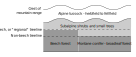
\includegraphics[width=\textwidth]{graphics/fig_090}
	\caption[Differences in zonation]{Differences in zonation near tree line where beech is present and where it is absent.}%
	\label{fig:90zonation}
\end{figure}

It seems more convenient to treat the higher altitude shrublands as one entity and for this reason I use the non-committal term `mountain shrublands'.

\section{Mountain Shrublands}

Where the mountain shrubland zone is dense and extensive\figureref{\fullref{fig:91shrubland}} it is easy to be impressed both by the variety of species present and by their range in leaf form (from large and leathery to needle-or scale-like) and in colour (from dark green to yellow-green or even orange-red).
\begin{SCfigure}[2.0][!b]
	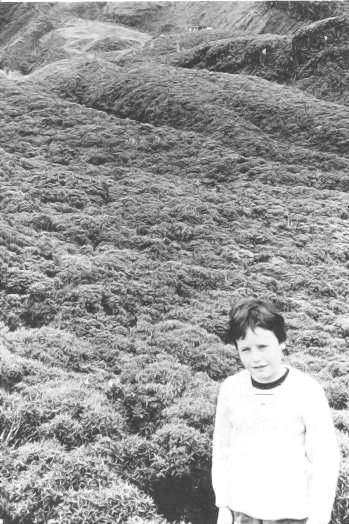
\includegraphics[width=0.33\textwidth]{graphics/fig_091}
	\caption[Mountain shrubland on Mt. Taranaki]{Mountain shrubland on Mt. Taranaki (Egmont).
	Beech (\BotanicRef{Nothofagus}) forest does not occur on this mountain.
	Photo: J. W. Dawson.}%
	\label{fig:91shrubland}
\end{SCfigure}
Unfortunately, if no tracks are present, this pleasing first impression may soon be dissipated by the discomforts and frustrations of trying to make progress.
The branches of some of the larger shrubs lie on and branch over the ground for considerable distances, so one alternates between trying to push through and between them and attempting to scramble over their tops.
After perhaps hours of snail-like progress it is a great relief to reach the open alpine vegetation above or the forest below.

\section{Subalpine Shrubs or Small Trees}

In the lower or subalpine parts of the shrub zone the species composition depends on soils and aspect.
In the Westland beech gap Wardle\footnote{\cite{wardle1977plant}} recognises a number of subalpine low forest or shrub communities which are in part typical for New Zealand as a whole.
They include:

\subsection[Mountain Lacebark (\emph{Hoheria glabrata}) low forest]{\IDX{Mountain Lacebark}[mountain lacebark] (\BotanicRef{Hoheria glabrata}[Hoheria][glabrata]) low forest}

\IDX{Mountain lacebark}[mountain lacebark] (\BotanicRef{Hoheria glabrata}[Hoheria][glabrata]) colonises young, deep, moist, well-drained and often stony soils such as those provided by slips, talus slopes and alluvial fans.
This small tree, being one of the few in New Zealand that is strongly deciduous, has attractive yellow to red leaves in the autumn.
Its clusters of white flowers, each up to \SI{4}{\centi\metre} across, are also a striking feature.
\IDX{Mountain holly}[mountain holly] (\BotanicRef{Olearia ilicifolia}[Olearia][ilicifolia]) also contributes to the canopy and the ground beneath has a dense cover of the \IDX{prickly shield fern} (\BotanicRef{Polystichum vestitum}[Polystichum][vestitum]).

\subsection[\emph{Dracophyllum}-\emph{Olearia} Low Forest and Scrub]{\BotanicRef{Dracophyllum}-\BotanicRef{Olearia} Low Forest and Scrub}

This occupies similar but older sites than \IDX{mountain lacebark} (\BotanicRef{Hoheria glabrata}[Hoheria][glabrata]) low forest.
Dominance is shared by the \IDX{mountain lacebark} (low forest only), \IDX{inanga} (\BotanicRef{Dracophyllum longifolium}[Dracophyllum][longifolium], scrub only), \IDX{mountain neinei} (\BotanicRef{Dracophyllum traversii}[Dracophyllum][traversii]) and \IDX{lancewood tree daisy} (\BotanicRef{Olearia lacunosa}[Olearia][lacunosa]), the last two being up to \SI{7}{\metre} tall.
The genus \BotanicRef{Dracophyllum}, although belonging to the dicotyledon class of the flowering plants has long, narrow, parallel-veined leaves similar, in the larger examples, to those of such monocotyledons as the \IDX{cabbage tree} (\BotanicRef{Cordyline australis}[Cordyline][australis]) or even the pineapple.
Indeed, mountain groves of \IDX{mountain neinei} (\BotanicRef{Dracophyllum traversii}[Dracophyllum][traversii]) are sometimes known locally as `pineapple forests'.
This species with its candelabra-like form, and its sword-like leaves forming a deep litter on the forest floor, is certainly the most distinctive member of the community.

At higher altitudes in the south-west of the South Island \IDX{mountain neinei} (\BotanicRef{Dracophyllum traversii}[Dracophyllum][traversii]) is replaced by the smaller \BotanicRef{Dracophyllum menziesii}[Dracophyllum][menziesii] and the equally distinctive \BotanicRef{Dracophyllum fiordense}[Dracophyllum][fiordense], which has an often unbranched trunk up to \SI{2}{\metre} high topped by an almost spherical mop of strongly downwardly curved leaves\figureref{\fullref{fig:92dracophyllum}}.
\IDX{Inanga}[inanga] (\BotanicRef{Dracophyllum longifolium}[Dracophyllum][longifolium]) is one of many shrub species with smaller needle leaves and a heath-like appearance.
Indeed the family to which \BotanicRef{Dracophyllum} belongs, Epacridaceae, is closely related to the heath family, Ericaceae.

\begin{SCfigure}[1.0][t]
	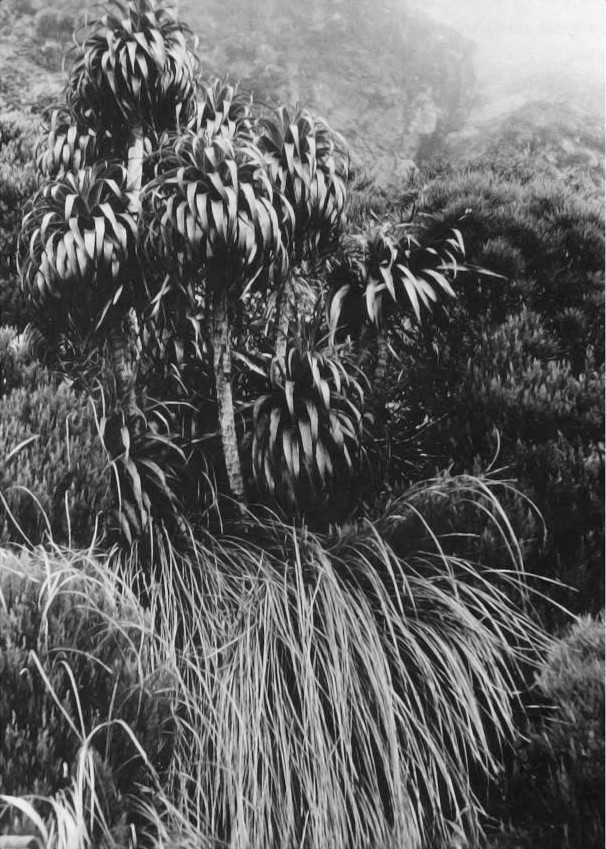
\includegraphics[width=0.5\textwidth]{graphics/fig_092}
	\centering
	\caption[A group of unbranched shrubs of \emph{Dracophyllum fiordense}]{A group of unbranched shrubs of \BotanicRef{Dracophyllum fiordense}[Dracophyllum][fiordense] together with needle-leaved Dracophyllums and other shrubs.
	The grass is \IDX{broadleaved snow tussock} (\BotanicRef{Chionochloa flavescens}[Chionochloa][flavescens]).
	Fiordland.
	Photo: Jane Maxwell.}%
	\label{fig:92dracophyllum}
\end{SCfigure}

\BotanicRef{Olearia lacunosa}[Olearia][lacunosa] also has narrow, although net-veined leaves, which are somewhat like those of juvenile \IDX{lancewood} (\BotanicRef{Pseudopanax crassifolius}[Pseudopanax][crassifolius]).
Some of the other shrub species with relatively large thick leaves are \IDX{broadleaf} (\BotanicRef{Griselinia littoralis}[Griselinia][littoralis]), mountain \IDX{five-finger} (\BotanicRef{Pseudopanax colensoi}[Pseudopanax][colensoi]) and \IDX{leatherwood} (\BotanicRef{Olearia colensoi}[Olearia][colensoi]).
\IDX{Haumakoroa}[haumakoroa] (\BotanicRef{Pseudopanax simplex}[Pseudopanax][simplex]) has somewhat smaller, thinner leaves and \IDX{weeping matipo} (\BotanicRef{Myrsine divaricata}[Myrsine][divaricata]) and \BotanicRef{Coprosma pseudocuneata}[Coprosma][pseudocuneata] have very small leaves.
Prominent ground plants are \IDX{small kiokio} (\BotanicRef{Blechnum procerum}[Blechnum][procerum]) and the tussock-like \IDX{mountain astelia} (\BotanicRef{Astelia nervosa}[Astelia][nervosa]).

Dominance of the shrub species varies from place to place in this community type, but it is at its most impenetrable where \IDX{leatherwood} (\BotanicRef{Olearia colensoi}[Olearia][colensoi]) with its stiff almost cardboard-like leaves predominates, as in the North Island ranges, the westernmost coastal ranges in the South Island and in Fiordland.

\subsection[Subalpine Heath-Scrub]{Subalpine Heath-Scrub\thinspace\footnote{\cite{burrows1979heathlands}}}

This occurs on old, leached infertile soils and is a low shrubbery from \SIrange{0.5}{1.5}{\metre} tall in which the small conifers \IDX{pink pine} (\BotanicRef{Halocarpus biformis}[Halocarpus][biformis]) and \IDX{mountain celery pine} (\BotanicRef{Phyllocladus aspleniifolius var.\ alpinus}[Phyllocladus][aspleniifolius var.\ alpinus]) share dominance with \IDX{leatherwood} (\BotanicRef{Olearia colensoi}[Olearia][colensoi]) and \IDX{inanga} (\BotanicRef{Dracophyllum longifolium}[Dracophyllum][longifolium]).

Both the conifers also occur in the lowlands of Westland where they become small trees.
In the greyish-green mountain celery pine, what appear to be fan-like or rhomboidal leaves are in fact flattened branchlets termed phylloclades.

These are some of the community types of subalpine shrubs and small trees, but there are a number of others related to special habitats or resulting from disturbances, whether caused by nature or by humans.
Many of the species of these communities may grow in the montane forests especially towards their upper limits.

\section{Alpine shrubs}

Above the actual or inferred treeline come shrubs that can be considered truly alpine, although many descend to lower altitudes in open habitats.
Immediately above treeline on moderate slopes with a reasonably well developed soil such shrubs generally intermingle with large tussock grasses and other herbs in what has been termed tussock-shrubland.
As altitude increases, the shrubs decrease and the herbs increase.
On steeper slopes, such as spurs and ridges, with shallow, stony soils, species of shrubs mostly different from those of the tussock-shrubland may form a more continuous cover, but there is usually a herb component.
On these rocky sites certain shrubs may extend to quite high altitudes, becoming shorter and more scattered as they do so.

It is in this higher shrubland zone that New Zealand's largest genus \BotanicRef{Hebe} attains its greatest prominence.
Of the approximately 60 commoner species of alpine shrubs 24 or 40 per cent are hebes, many of them exhibiting the symmetry of form and attractiveness of foliage --- grey-green, yellow-green and shades of yellow and orange --- that have made the genus so well known horticulturally in many parts of the world.
The alpine hebes can be divided into two approximately equal groups contrasting strongly in growth habit.
In the first group the leaves, although short and fairly broad, are spreading and often very precisely arranged in four vertical rows.
The shapes of such shrubs may be so symmetrical and their surfaces so dense, that they appear to have been trimmed to shape.
Appropriately, one of them has been named \BotanicRef{Hebe topiaria}[Hebe][topiaria].
The relationship of the hebes in this group with the willow-leaved species (\IDX{koromiko}s) of the lowlands is quite evident, but with the second group of so-called `whipcord' hebes this is not so; they resemble instead the quite unrelated scale-leaved conifers\figureref{\fullref{fig:93hebe}}.
It is no surprise to learn that one of them is named \IDX{cypress hebe} (\BotanicRef{Hebe cupressoides}[Hebe][cupressoides]).
Both growth forms are represented in tussock-shrubland and on stony ridges.

\begin{figure}[!ht]
	% Outer minipage scaled to limit width.
	% Inner minipages scaled so the images have the same height.
	\begin{minipage}[t]{\textwidth}
		\begin{minipage}[t]{(\textwidth-\fgap) * \real{0.5}}
			\centering
			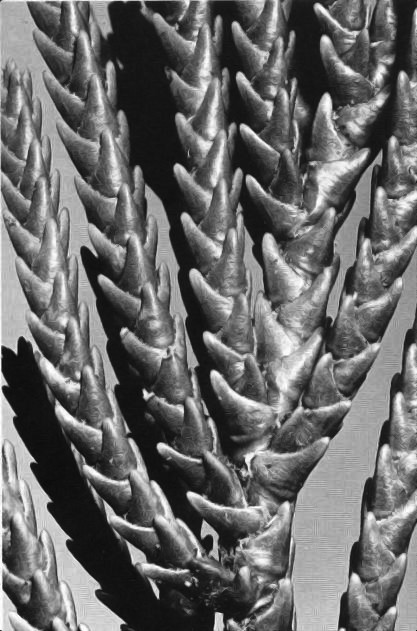
\includegraphics[width=\textwidth]{graphics/fig_093}
			\caption[\emph{Hebe tetragona}]{\BotanicRef{Hebe tetragona}[Hebe][tetragona].
			A `whipcord' Hebe.
			Photo: M. D. King.}%
			\label{fig:93hebe}
		\end{minipage}\hspace{\fgap}%
		\begin{minipage}[t]{(\textwidth-\fgap) * \real{0.5}}
			\centering
			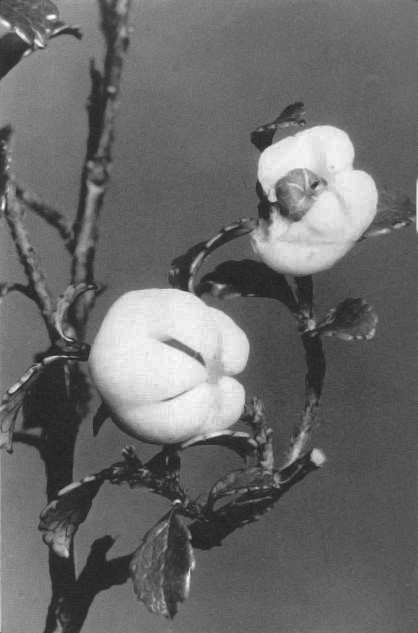
\includegraphics[width=\textwidth]{graphics/fig_094}
			\caption[\emph{Gaultheria depressa}]{\BotanicRef{Gaultheria depressa}[Gaultheria][depressa].
			The upper fruit has had part of the fleshy calyx removed to reveal the seed capsule.
			Photo: M. D. King.}%
			\label{fig:94gaultheria}
		\end{minipage}
	\end{minipage}
\end{figure}

Similar in general appearance to the hebes with spreading four-ranked leaves are a number of species of \BotanicRef{Pimelea} or New Zealand `daphnes'.
The flowers with their pairs of stamens are also quite Hebe-like, but as a general rule the two genera can be distinguished by the presence (\BotanicRef{Pimelea}) or absence (\BotanicRef{Hebe}) of leaf and flower hairs.
Pimelea leaves often feel quite silky to touch.
Pimeleas occur both in grassland and on rocks.

Most of the alpine dracophyllums have needle leaves.
Taller species in tussock-shrubland have a switch-like habit with narrow branching angles, others in similar habitats or on rocky ridges are more or less prostrate.
During the colder period of the year especially, the dracophyllums add colour to the alpine scene when their leaves develop bright reddish brown hues.

A few gaultherias belonging to the Ericaceae or heath family also occur in alpine communities.
\BotanicRef{Gaultheria crassa}[Gaultheria][crassa] is a shrub up to \SI{1}{\metre} high growing in a variety of sites.
The clusters of small white flowers are bell-like and not unlike those of the dracophyllums.
The leaves, however, are short, broad and quite thick.
\IDX{Snowberry}[snowberry] (\BotanicRef{Gaultheria depressa var.\ novae-zelandiae}[Gaultheria][depressa var.\ novae-zelandiae]) is a prostrate shrub in open places remarkable for its relatively large white, pink or red, berry-like fruits often referred to as `snow berries'.
The fleshy parts of the fruits are actually the persistent and enlarged sepals of the flowers\figureref{\fullref{fig:94gaultheria}}.
\IDX{Prostrate snowberry}[prostrate snowberry] (\BotanicRef{Pernettya macrostigma}[Pernettya][macrostigma]), which belongs to a genus closely related to \BotanicRef{Gaultheria}, is a scrambling, interlaced shrub of poorly drained areas in tussock grassland.
It has an even more remarkable fruit than that of \BotanicRef{Gaultheria depressa}[Gaultheria][depressa], as both the persistent sepals and the seed capsule within them are fleshy.
Natural hybrids between \BotanicRef{Pernettya macrostigma}[Pernettya][macrostigma] and a \BotanicRef{Gaultheria} have bright red fruits in which the plump sepals form a crown-like cup around the capsule.

All except one of the relatively few shrubby alpine coprosmas have very small leaves and slender twigs.
Three of these are prostrate and scrambling, \BotanicRef{Coprosma cheesemanii}[Coprosma][cheesemanii] and \BotanicRef{Coprosma crenulata}[Coprosma][crenulata] in damp places in tussock grassland and \BotanicRef{Coprosma depressa}[Coprosma][depressa]  on rocky sites.
\BotanicRef{Coprosma pseudocuneata}[Coprosma][pseudocuneata] with its attractive, strongly recurved, yellowish green leaves has an erect habit and extends to quite high altitudes in sheltered rocky sites.
The one large-leaved \BotanicRef{Coprosma}, \BotanicRef{Coprosma serrulata}[Coprosma][serrulata], grows in shaded tussock shrubland  and also on shaded rocky bluffs.
Its leaves are thick and leathery with prominent veins.

The Compositae or daisy family is represented by a few species belonging to three genera.

\BotanicRef{Brachyglottis bidwillii}[Brachyglottis][bidwillii] is widespread in tussock shrubland and on rocky bluffs.
Its leaves are rounded and very thick with a thick, felt like mass of hairs on their undersides.
Two other species are more localised, \BotanicRef{Brachyglottis adamsii}[Brachyglottis][adamsii] in adjacent parts of the North and South Islands, and \BotanicRef{Brachyglottis revolutus}[Brachyglottis][revolutus] in the south-west of the South Island.

The genus \BotanicRef{Helichrysum}, which includes the flowers known as `everlastings', has several shrubby alpine species in the drier eastern mountains of the South Island where they grow on rocky outcrops and ridges.
They all have a similar distinctive appearance with scale-like, but somewhat swollen, strongly convex leaves closely pressed to the stems.
The rounded backs of the leaves may be very shiny and each leaf is surrounded by a dense mass of white hairs.
The most robust and striking species is  \IDX{coral sea shrub} (\BotanicRef{Helichrysum coralloides}[Helichrysum][coralloides]) with cylindrical stems up to \SI{1}{\centi\metre} in diameter.

\IDX{Tauhinu}[tauhinu] (\BotanicRef{Cassinia vauvilliersii}[Cassinia][vauvilliersii]) may be common in tussock-shrubland throughout New Zealand as well as in open vegetation at lower altitudes.
It is an erect shrub, often with a distinct yellowish colouration from the hairs on the undersides of the small leaves.

\IDX{Porcupine shrub}[porcupine shrub] (\BotanicRef{Melicytus alpinus}[Melicytus][alpinus], Hymenanthera) of the violet family is a small shrub with short, stiff, interlacing twigs which are almost spiny at the tips.
The species occurs throughout the South Island and is most frequent on rocky ridges and outcrops.

\IDX{Creeping matipo}[creeping matipo] (\BotanicRef{Myrsine nummularia}[Myrsine][nummularia]) is a small-leaved, prostrate, thin-stemmed shrub found throughout the New Zealand mountains where it favours rock outcrops and open places in tussock grassland.
Its most striking feature is the bright violet-blue colouration of the berries.

Three dwarf conifers may be frequent throughout tussock shrubland.
\IDX{Snow totara}[snow totara] (\BotanicRef{Podocarpus nivalis}[Podocarpus][nivalis]) forms low bushes in this community, but is also common at scree margins and on moraines at lower elevations.
The \IDX{pygmy pine} (\BotanicRef{Lepidothamnus laxifolius}[Lepidothamnus][laxifolius]), sometimes called the smallest conifer in the world, forms even lower mat-like patches in poorly drained sites and the \IDX{mountain celery pine} (\BotanicRef{Phyllocladus aspleniifolius var.\ alpinus}[Phyllocladus][aspleniifolius var.\ alpinus]) is still erect in habit though shorter than it is in the subalpine shrublands.

\section[Tussock Herbfield]{Tussock Herbfield\thinspace\footnote{\cite{mark1980progress}}}

This type of alpine vegetation occupies a zone about \SI{500}{\metre} wide above the treeline where soils of adequate depth are present.
The term `herb-field' as applied to northern hemisphere mountains is defined as a complete cover of herbaceous alpine plants, but in New Zealand the modified term tussock herbfield is preferred.
This is because the dominant and conspicuous large tussock grasses belonging to the genus \BotanicRef{Chionochloa}\figureref{\fullref{fig:95red-tussock}, \fullref{fig:96snow-tussock}}, although they lack woody tissues, are often as tall as or taller than some of the alpine shrubs.

\begin{SCfigure}[1.0][!b]
	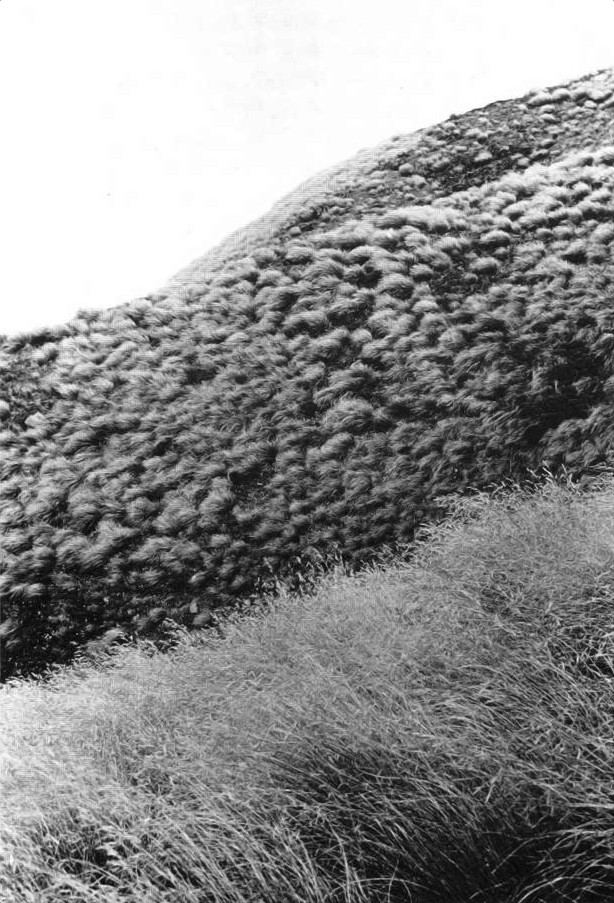
\includegraphics[width=0.5\textwidth]{graphics/fig_095}
	\centering
	\caption[Red tussock grassland on Mt. Taranaki]{Red tussock grassland on Mt. Taranaki (Egmont).
	Tussocks with seed heads in foreground.
	Photo: J. W. Dawson.}%
	\label{fig:95red-tussock}
\end{SCfigure}

\begin{SCfigure}[1.0][t]
	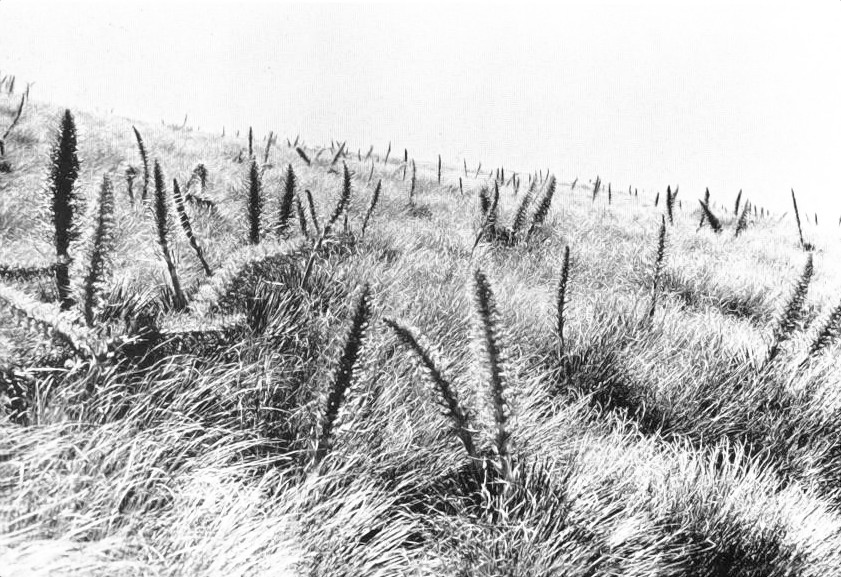
\includegraphics[width=0.66\textwidth]{graphics/fig_096}
	\centering
	\caption[Snow tussock]{The \IDX{snow tussock} (\BotanicRef{Chionochloa macra}[Chionochloa][macra]) with flower heads of the spaniard (\BotanicRef{Aciphylla scott-thomsonii}[Aciphylla][scott-thomsonii]).
	Old Man Range, Otago.
	Photo: J. W. Dawson.}%
	\label{fig:96snow-tussock}
\end{SCfigure}

\subsection{Snowgrasses}

The larger alpine tussock grasses, or `snow grasses' as they are called, are frequently a metre high and sometimes as wide.
Under good conditions they may reach head height at up to \SI{2}{\metre}.
Growth is slow and some of the larger specimens are estimated to be several centuries old.\footnote{\cite{mark1974snow}}
The more or less hemispherical form of many of the \IDX{snow tussock}s confers on the mountain slopes a very distinctive and attractive texture reminiscent of that of cirrus clouds or, when the tussocks are tossed by the wind, waves of the sea.
The colour of a \IDX{snow tussock} landscape is generally not green, but, depending on the species, ranges from a pale straw colour through shades of brown to a distinctly reddish shade.
The lack of greenness results partly from the regular dying back of the leaves from the tips and partly to the presence of masking pigments.
Heavy flowering seasons of the snow grasses are sporadic and often coincide with those of the beech species.
This suggests that snow grasses too require a warm summer preceding flowering for the initiation of flower buds.

The flower and seed heads of some of the larger \IDX{snow tussock}s are quite diffuse, and their very slender stems and small, scattered, pale, flower or seed heads give an insubstantial misty effect similar to that of the garden \BotanicRef{Gypsophila}, so popular in flower arrangements.
On the wetter western mountains of the South Island the \IDX{broadleaved snow tussock}[tussock!snow!broadleaved] (\BotanicRef{Chionochloa flavescens}[Chionochloa][flavescens]), can grow sometimes \SI{2}{\metre} high, and dominates in the zone \SI{200}{\metre} above treeline.
The \IDX{mid-ribbed snow tussock}[tussock!snow!mid-ribbed] (\BotanicRef{Chionochloa pallens}[Chionochloa][pallens]) is often present, generally on younger, better drained soils.
Both species are also common on the North Island axial ranges.
With increasing altitude on the wet South Island mountains the two large \IDX{snow tussock}s gradually give way to the much smaller \IDX{curled snow tussock}[tussock!snow!curled] (\BotanicRef{Chionochloa crassiuscula}[Chionochloa][crassiuscula]).

On Mt. Taranaki (Egmont) and the central volcanoes in the North Island the only \IDX{snow tussock} present is \IDX{red tussock} (\BotanicRef{Chionochloa rubra}[Chionochloa][rubra]), which occupies a wide range of habitats in the herbfield zone.
In the South Island on the wetter mountains \IDX{red tussock} is abundant only at or below the treeline on poorly drained and frosty flat valley floors.
With its large size and strong reddish colouration it provides an impressive sight\figureref{\fullref{fig:97red-tussock}}.

\begin{SCfigure}[1.0][!b]
	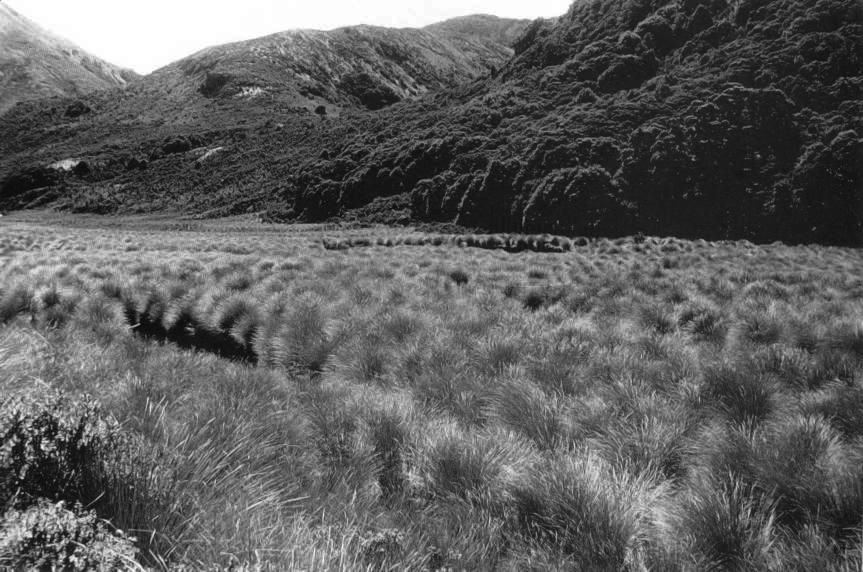
\includegraphics[width=0.66\textwidth]{graphics/fig_097}
	\centering
	\caption[Red tussock]{Dense cover of \IDX{red tussock} (\BotanicRef{Chionochloa rubra}[Chionochloa][rubra]) on a swampy valley floor.
	Near Boulder Lake, north-west Nelson.
	Photo: J. W. Dawson.}%
	\label{fig:97red-tussock}
\end{SCfigure}

On the drier eastern South Island mountains in the southern half, the dominant snow tussock in the low alpine zone is the \IDX{narrow-leaved snow tussock}[tussock!snow!narrow-leaved] (\BotanicRef{Chionochloa rigida}[Chionochloa][rigida]).
This gives way at higher altitudes to the smaller recently described slim snow tussock (\BotanicRef{Chionochloa macra}[Chionochloa][macra]).
Only slim snow tussock extends north of the central South Island and it then occupies a broader altitudinal zone.

Among the smaller species of \BotanicRef{Chionochloa}, which are found mostly at higher levels in herbfield, \IDX{carpet grass} (\BotanicRef{Chionochloa australis}[Chionochloa][australis]) is worth a special mention.
As its common name indicates it does not have a tussock habit, but forms thick, often extensive swards.
The needle-like leaves are dark green and shiny and as they are also slippery and tend to lie downhill, they need to be walked on with care.
Carpet grass is found on wetter mountains in the northern third of the South Island.

Where snow tussocks are tall and dense near the treeline one might think there would be little room left for other alpine herbs; in fact there are quite a number.
Some are small and inconspicuous, enjoying the shelter and tolerating the shade of the tussocks.
Others are much more conspicuous and could be termed large or even giant herbs approaching or exceeding the tussocks in height.

\subsection{Spaniards}

Notable among the large alpine herbs are the Spaniards or speargrasses belonging to the genus \BotanicRef{Aciphylla} of the Umbelliferae (carrot family).\footnote{\cite{dawson1978research}}
Nothing could look more unlike a carrot plant than the larger spaniards of tall tussock grassland.
In their tussock-like clumps the large leaves are deeply divided into hard, rigid segments tipped by needle-sharp spines.
The flower, and later seed, heads are equally unusual in that, instead of being broad and open as is more typical for the family, they are dense, narrow and lance-like.
The individual flower clusters, densely aggregated on the upper parts of the lances, are exceeded in length by their associated bracts.
These bracts have segments as spiny as those of the leaves.
Having suffered while collecting specimens of such spaniards for study, I am inclined to agree with the suggestion that the excessive spininess is a defence against browsing animals (and botanists), which in pre-human times in New Zealand would have been the moas.
However, despite their unpleasant characteristics, many of the spaniards are striking in appearance and, when strongly coloured, decidedly handsome as well.
Some species have grey-green leaves and flower heads ranging from green to pale yellow, others have both leaves and flower heads with a quite strong yellow to orange colouration as, for example, in the \IDX{golden spaniard} (\BotanicRef{Aciphylla aurea}[Aciphylla][aurea])\figureref{\fullref{fig:98golden-spaniard}}.

\begin{SCfigure}[1.0][!b]
	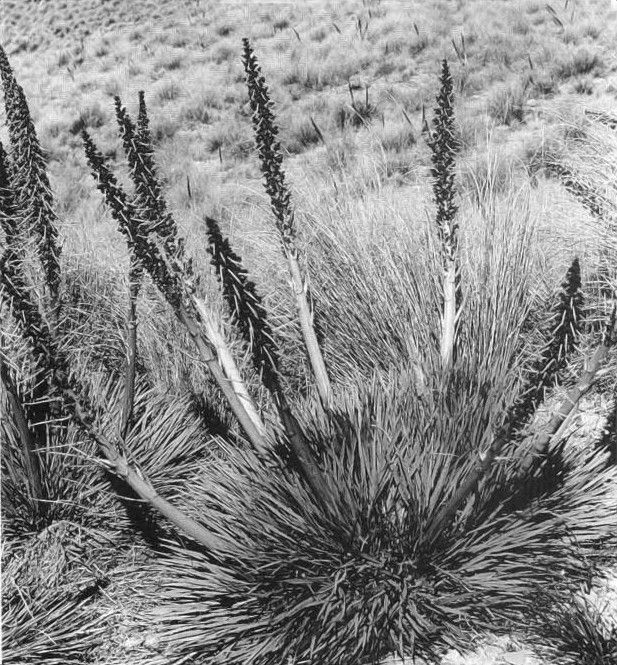
\includegraphics[width=0.5\textwidth]{graphics/fig_098}
	\centering
	\caption[The golden spaniard]{The golden spaniard (\BotanicRef{Aciphylla aurea}[Aciphylla][aurea]) scattered through tussock grassland comprised of \IDX{narrow-leaved snow tussock}[tussock!snow!narrow-leaved] (\BotanicRef{Chionochloa rigida}[Chionochloa][rigida]). Mt. St.\ Bathans, Otago.
	Photo: J. W. Dawson.}%
	\label{fig:98golden-spaniard}
\end{SCfigure}

Most of the large species of spaniard grow in moist tussock herbfield or open mountain shrubland.
In the very wet south west of the South Island is the appropriately named \BotanicRef{Aciphylla horrida}[Aciphylla][horrida].
Further east, but still in moist situations, the grey-green \IDX{giant speargrass} (\BotanicRef{Aciphylla scott-thomsonii}[Aciphylla][scott-thomsonii]) is prominent\figureref{\fullref{fig:96snow-tussock}}.
This species has the distinction of being the largest, with seed heads sometimes as much as \SI{4}{\metre} high.
Other large species occur further north with a few extending through the North Island ranges.
One of the latter, \BotanicRef{Aciphylla colensoi}[Aciphylla][colensoi], is notable for the bright yellow to orange midribs of its leaf segments.

The \IDX{golden spaniard} (\BotanicRef{Aciphylla aurea}[Aciphylla][aurea]), is often prominent in drier habitats in the eastern South Island and is characteristic of \IDX{narrow-leaved snow tussock}[tussock!snow!narrow-leaved] grassland\figureref{\fullref{fig:98golden-spaniard}}.
In higher herbfield where the plant cover is shorter the larger species of \BotanicRef{Aciphylla} give way to smaller forms.
Some of the smaller forms are spiny with narrow inflorescences; others are more like the related \BotanicRef{Anisotome} with soft leaves and broad inflorescences.

It is difficult to understand why narrow dense inflorescences should have evolved in \BotanicRef{Aciphylla}.
It could be seen as a protective device as the short flower clusters are readily shielded by the spinescent bracts, but similar (although not spiny) inflorescences occur in quite unrelated plants elsewhere in the world --- the tree Senecios and Lobelias of the central African Mountains, the \BotanicRef{Puya} (Bromeliaceae) of the northern Andes, \BotanicRef{Echium} in the Canary Islands and the grass trees (\BotanicRef{Xanthorrhea}) in Australia, to name a few.

\subsection[Mountain Buttercups]{Mountain Buttercups\thinspace\footnote{\cite{fisher1965alpine}}}

The largest and best known of these is \BotanicRef{Ranunculus lyallii}[Ranunculus][lyallii], the so called `\IDX{Mount Cook Lily}[Mount Cook lily]'.
It seems that any large herb, especially if it has large, white flowers, as in this case, is inevitably and often erroneously termed a `lily'.
\BotanicRef{Ranunculus lyallii}[Ranunculus][lyallii] is most admired for its large, pure-white flowers up to \SI{6}{\centi\metre} across\figureref{\fullref{fig:99ranunculus}}.
\begin{SCfigure}[2.0][!b]
	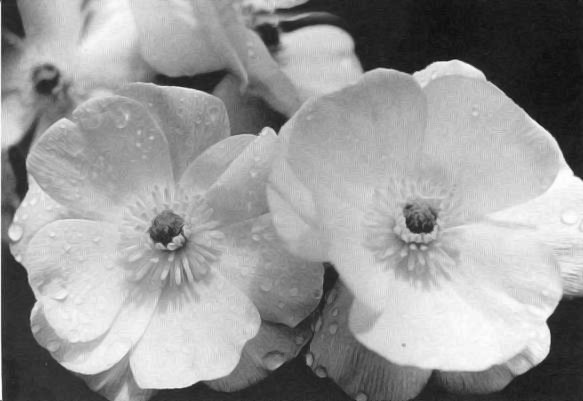
\includegraphics[width=0.5\textwidth]{graphics/fig_099}
	\centering
	\caption[Flowers of \emph{Ranunculus lyallii}]{Flowers of \BotanicRef{Ranunculus lyallii}[Ranunculus][lyallii] at Arthurs Pass, Canterbury.
	Photo: J. W. Dawson.}%
	\label{fig:99ranunculus}
\end{SCfigure}
It is equally remarkable for its large, rather floppy, almost circular leaves up to \SI{30}{\centi\metre} in diameter\figureref{\fullref{fig:100alpine-plants}}.
\begin{SCfigure}[2.0][t]
	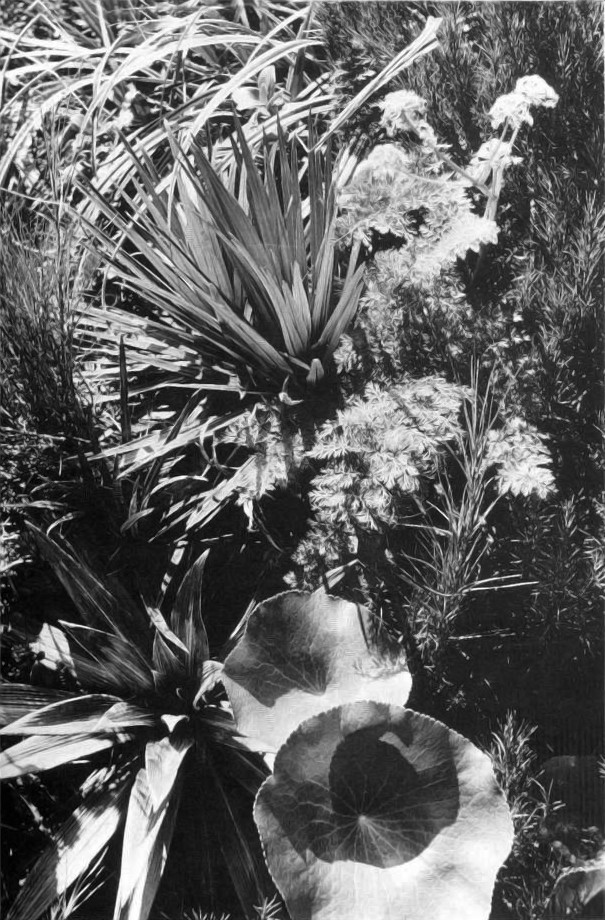
\includegraphics[width=0.5\textwidth]{graphics/fig_100}
	\centering
	\caption[Alpine plants at Arthurs Pass]{Group of alpine plants at Arthurs Pass, Canterbury.
	The large circular leaves are \BotanicRef{Ranunculus lyallii}[Ranunculus][lyallii].
	Two mountain daisies are present, \BotanicRef{Celmisia semicordata}[Celmisia][semicordata] below and \BotanicRef{Celmisia armstrongii}[Celmisia][armstrongii] above.\IDX{mountain daisy}
	The herb with very divided leaves is \IDX{Haasts carrot}s (\BotanicRef{Anisotome haastii}[Anisotome][haastii]) and the long silvery leaves at the top belong to the \IDX{mountain astelia} (\BotanicRef{Astelia nervosa}[Astelia][nervosa]).
	The needle-leaved shrubs are \IDX{inanga} (\BotanicRef{Dracophyllum longifolium}[Dracophyllum][longifolium]).
	Photo: J. W. Dawson.}%
	\label{fig:100alpine-plants}
\end{SCfigure}
Plants of this species may reach \SI{1}{\metre} in height among tussocks or shrubs, particularly in moist places, throughout the South Island mountains, except in the far north, and in Fiordland.
Other smaller, but still large, species have bright buttercup yellow flowers, for example the variable \IDX{korikori} (\BotanicRef{Ranunculus insignis}[Ranunculus][insignis]) throughout the axial ranges of the North Island and in the northern half of the South Island and \IDX{mountain buttercup} (\BotanicRef{Ranunculus nivicola}[Ranunculus][nivicola]) in the tussock herbfield of Mt. Taranaki (Egmont) and also on the central North Island mountains.
\BotanicRef{Ranunculus verticillatus}[Ranunculus][verticillatus], which is also yellow-flowered, is more slender and less conspicuous, but nevertheless common in the southern North Island and northern South Island.
It often grows through, and is supported by, shrubs and snow tussocks.

\subsection{Ourisia}

The Ourisias are sometimes called mountain foxgloves.
This is a common name with at least some validity since foxgloves and \BotanicRef{Ourisia} belong to the same family, the Scrophulariaceae.

The two large species of \BotanicRef{Ourisia} found in tussock herbfield, like the large \BotanicRef{Ranunculus} species, have leathery or somewhat fleshy, dark green leaves.
The flowers are white with yellow centres, \SIrange{2}{3}{\centi\metre} across and have the five petals fused at the base.
The flowers are distinctively arranged in spreading circles or whorls, one above the other.
\IDX{Mountain foxglove}[mountain foxglove] (\BotanicRef{Ourisia macrophylla}[Ourisia][macrophylla]) with two subspecies is found on wetter mountains in the North Island and \IDX{snowy mountain foxglove} (\BotanicRef{Ourisia macrocarpa}[Ourisia][macrocarpa]) also with two subspecies in similar sites throughout the South Island.

\subsection{Gentians}

To those familiar with the brilliantly blue, deeply bell-shaped gentians of the northern hemisphere, the New Zealand versions must come as a surprise.
Their flowers are like sprinklings of snow among the tussocks and in each flower the petals are much more deeply divided than those of northern species although still fused near the base\figureref{\fullref{fig:101gentiana}}.
The leaves are generally somewhat fleshy and sometimes both leaves and stems have a strong red or purple colouration masking the green.
\begin{SCfigure}[2.0][!b]
	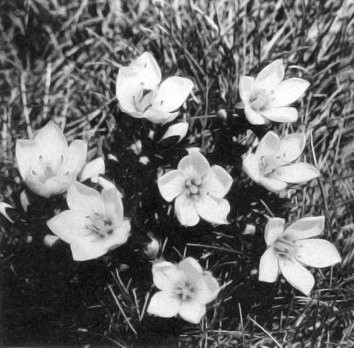
\includegraphics[width=0.5\textwidth]{graphics/fig_101}
	\centering
	\caption[\emph{Gentiana bellidifolia}]{\BotanicRef{Gentiana bellidifolia}[Gentiana][bellidifolia].
	Mt. Peel,  N. W. Nelson.
	Photo: J. W. Dawson.}%
	\label{fig:101gentiana}
\end{SCfigure}
The flowers are usually pure white, but sometimes have purple veins.
The distinctions between many of the New Zealand species are still not clear, but several are prominent in tussock herbfield and shrubland.
\IDX{Grassland gentian}[grassland gentian] (\BotanicRef{Gentiana corymbifera}[Gentiana][corymbifera]) can be up to half a metre tall and is mostly found in drier eastern tussock grassland throughout the South Island mountains.
The similar \BotanicRef{Gentiana montana}[Gentiana][montana] is widespread in the wetter, mostly western mountains of the South Island and in Fiordland.
\BotanicRef{Gentiana bellidifolia}[Gentiana][bellidifolia], a somewhat smaller species, ranges throughout the mountains of both North and South Islands.

\subsection[Mountain Daisies]{Mountain Daisies\thinspace\footnote{\cite{given1969synopsis}}}

Mountain daisies or celmisias are probably the most frequently encountered of our alpine herbs\figureref{\fullref{fig:102celmisias}}.
\begin{SCfigure}[1.0][t]
	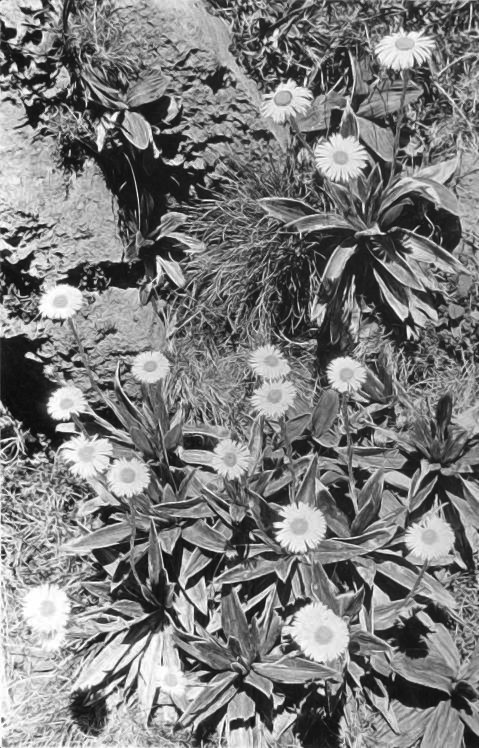
\includegraphics[width=0.5\textwidth]{graphics/fig_102}
	\centering
	\caption[A group of celmisias in flower]{A group of celmisias in flower --- \BotanicRef{Celmisia semicordata}[Celmisia][semicordata].
	There are a few non-flowering rosettes of \BotanicRef{Celmisia traversii}[Celmisia][traversii] also.
	Mt. Arthur,  N. W. Nelson.
	Photo: J. W. Dawson.}%
	\label{fig:102celmisias}
\end{SCfigure}
In other genera, two or three species may occur together at the same locality.
Celmisias may have as many as five or six species occurring together.
As befits the family Compositae, \BotanicRef{Celmisia} flowers\footnote{What is generally called a flower in the Compositae is really a very condensed inflorescence (capitulum) comprising many small flowers.} are daisy-like and white with yellow to orange centres.
In some species they may measure up to 7 or 8 or even \SI{10}{\centi\metre} in diameter, The leaves are more diverse and remarkable than the flowers.
In some species they are thin and soft in texture and sometimes sticky, but in many others they are very firm with hard upper surfaces and in colour range from grey-green through yellow-green to dark green.
The most notable and attractive feature of many \BotanicRef{Celmisia} leaves is a dense and often thick felt of hairs on the undersides and sometimes the upper sides as well.
This tomentum, as it is termed, may be pure white, cream to buff or even bright rusty brown.

Some celmisias of tussock herbfield have their leaves in one or more rosettes close to the ground.
Others, which form in patches, have closely branched, spreading stems with more dispersed leaves.
The stems of some of the latter can be fairly woody, and when they are semi-erect, the plants could be described as dwarf shrubs.

\BotanicRef{Celmisia semicordata}[Celmisia][semicordata]\figureref{\fullref{fig:102celmisias}} has the largest leaves and flowers of the genus.
The leaves are in large rosettes and are silvery green with white undersides.
The species is common in both open shrubland and tussock herbfield on wetter mountains throughout the South Island except the far north.
\BotanicRef{Celmisia verbascifolia}[Celmisia][verbascifolia], with a similar range to \BotanicRef{Celmisia semicordata}[Celmisia][semicordata], and \BotanicRef{Celmisia traversii}[Celmisia][traversii]  in the north-west and south-west of the South Island are similar in habit, but somewhat smaller than \BotanicRef{Celmisia semicordata}[Celmisia][semicordata].
\BotanicRef{Celmisia verbascifolia}[Celmisia][verbascifolia] is notable for the bright purple petioles and midribs of its leaves and \BotanicRef{Celmisia traversii}[Celmisia][traversii] for the deep, velvety rusty red tomentum on the leaf undersides.
The commonest \BotanicRef{Celmisia} in New Zealand is \BotanicRef{Celmisia spectabilis}[Celmisia][spectabilis], which in some of its forms is like a small \BotanicRef{Celmisia semicordata}[Celmisia][semicordata].
It occurs throughout the mountains of the North and the northern half of the South Island in both wet and dry tussock grassland.
It becomes particularly abundant following fires.

Three species are similar in having tufts of long, narrow, pointed sword-like leaves, which leads to them sometimes being mistaken for spaniards (\BotanicRef{Aciphylla}).
\IDX{False spaniard}[false spaniard] (\BotanicRef{Celmisia lyallii}[Celmisia][lyallii]) ranges along the eastern sides of the South Island mountains in \IDX{slim snow tussock} (\BotanicRef{Chionochloa macra}[Chionochloa][macra]) grassland, and \IDX{Petrie’s mountain daisy} (\BotanicRef{Celmisia petriei}[Celmisia][petriei]) and \IDX{Armstrong’s mountain daisy} (\BotanicRef{Celmisia armstrongii}[Celmisia][armstrongii]) together span the wetter western mountains of the South Island, \BotanicRef{Celmisia petriei}[Celmisia][petriei] in the north-west and south-west and \BotanicRef{Celmisia armstrongii}[Celmisia][armstrongii] in between.

Of the many smaller leaved species which form spreading mats a metre or more in diameter, \IDX{white mountain daisy} (\BotanicRef{Celmisia incana}[Celmisia][incana]) is probably the most striking as it often has a completely white tomentum of hairs on both sides of the leaves as well as the flower stems.
It ranges throughout the North Island mountains and continues to the middle of the South Island.

Three genera of monocotyledons other than grasses may also be prominent in tussock herbfield and shrubland.

\subsection{Bulbinella}

Species of this genus may be abundant on moist, shady slopes in tussock herbfield, their heads of starry yellow flowers often providing something unusual in New Zealand mountain landscapes --- a mass of solid colour.
Their leaves are tufted and long and narrow.
\BotanicRef{Bulbinella hookeri}[Bulbinella][hookeri] ranges from the North Island mountains to north Canterbury; \BotanicRef{Bulbinella angustifolia}[Bulbinella][angustifolia], sometimes inappropriately known as `Maori onion', ranges through the drier eastern mountains of the South Island from North Canterbury southwards; and \BotanicRef{Bulbinella gibbsii}[Bulbinella][gibbsii] in the wetter mountains of the southern North Island, southern South Island and Fiordland.

\subsection{Mountain Flax}

The term `flax' for the genus \BotanicRef{Phormium}, although firmly established, is yet another inappropriate common name as \BotanicRef{Phormium} and the true linen flax (\BotanicRef{Linum}) have in common only the possession of useful fibres.
\IDX{Mountain flax}[mountain flax] or \IDX{wharariki} is \BotanicRef{Phormium cookianum}[Phormium][cookianum] and its tufts of narrow, leathery leaves may be conspicuous in poorly drained places in tussock herbfield and shrubland.
The flowers in its quite tall heads vary in colour, from plant to plant, from yellow to dark reddish purple.

\subsection{Astelia}

The thirteen New Zealand species of \BotanicRef{Astelia} are about equally divided between the forests and the mountains.
The flower heads of the smaller alpine species are short and inconspicuous, but their bright red to orange berries are strikingly attractive.
Two large species may be conspicuous in wet places in tussock herbfield and shrubland.
\IDX{Mountain astelia}[mountain astelia] (\BotanicRef{Astelia nervosa}[Astelia][nervosa]\figureref{\fullref{fig:103astelia}}) is found throughout the country, has tufts of leaves up to a metre or more in length, varying from pale green to silvery white.
\begin{SCfigure}[1.0][!b]
	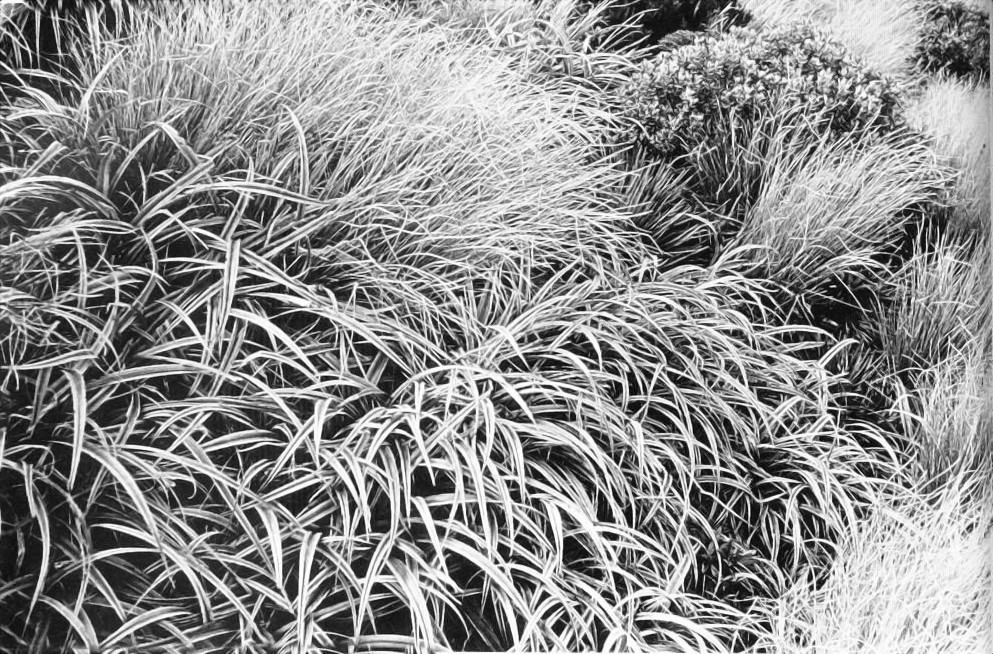
\includegraphics[width=0.66\textwidth]{graphics/fig_103}
	\centering
	\caption[\emph{Astelia nervosa} in snow tussock]{\BotanicRef{Astelia nervosa}[Astelia][nervosa] in snow tussock (\BotanicRef{Chionochloa pallens}[Chionochloa][pallens]) grassland.
	Mt. Holdsworth, southern North Island.
	Photo: J. W. Dawson.}%
	\label{fig:103astelia}
\end{SCfigure}
In the latter case the leaves look as if covered with frost.
\BotanicRef{Astelia petriei}[Astelia][petriei], with shorter, broader, pale green leaves, grows on the higher rainfall mountains of the western South Island.
The smaller, patch-forming \BotanicRef{Astelia nivicola}[Astelia][nivicola] has a similar range but at higher altitudes in herbfield.
The smallest herbfield species is the grasslike \BotanicRef{Astelia graminea}[Astelia][graminea], which is especially common among \IDX{carpet grass} (\BotanicRef{Chionochloa australis}[Chionochloa][australis]) in the northern South Island.

\section[Cushion Bogs]{Cushion Bogs\thinspace\footnote{\cite{gibson1985comparison}}}

Bogs develop in the subalpine and low alpine zones where drainage is poor.\footnote{Cushion bogs are also found at sea level on the south coast of the South Island near Invercargill.}
Suitable sites are hollows formed by glaciers and flat areas under high rainfall conditions on glacial terraces, mountain passes and flat topped mountain ridges.
Where rainfall is high, rain may provide most of the water in the bogs, but in drier eastern areas drainage from the surrounding slopes makes the major contribution.
When the water table is near the surface, the dominant plants in the bogs are of cushion form.
Cushion plants are freely but closely branched; and the ultimate twigs, with their upper living and lower dead leaves, are so closely pressed together lengthwise that the exposed tips of the living leaves form a firm, continuous, often unyielding surface.
Many cushion plants can be stood on without suffering any visible effects.
The leaf tips of each ultimate branchlet may form a circular pattern or be compressed into an hexagonal shape.
Depending on the species the cushions range from a few centimetres to a metre or more in diameter.
They are broadly convex to almost hemispherical in form and are separated by shallow to quite deep hollows.

A number of sedges and related plants occur in mountain bogs throughout the country.
The \BotanicRef{Centrolepis} and \BotanicRef{Gaimardia} species form soft moss-like cushions; \IDX{comb sedge} (\BotanicRef{Oreobolus pectinatus}[Oreobolus][pectinatus]) with its leaves distinctively arranged in two rows in one plane forms a firmer cushion while other species of the genus form flat mats.
Of other cushion plants, \BotanicRef{Donatia novae-zelandiae}[Donatia][novae-zelandiae] forms much larger, broadly convex, extremely dense cushions whose dark green leaf tips contrast strongly with the numerous, small white flowers in season\figureref{\fullref{fig:104donatio}}.
\begin{SCfigure}[1.0][!b]
	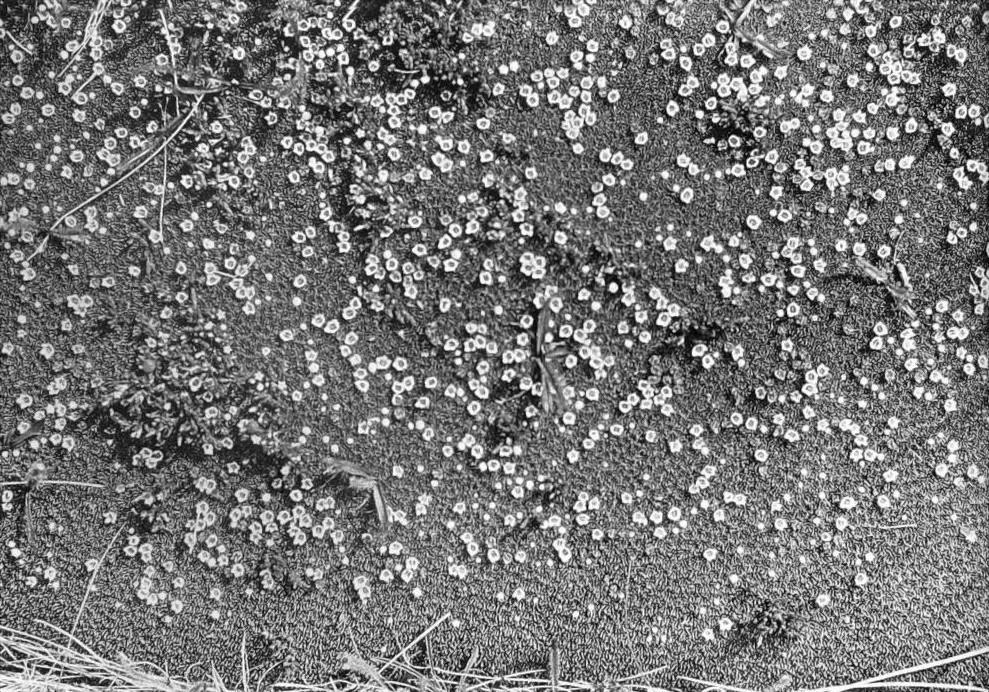
\includegraphics[width=0.66\textwidth]{graphics/fig_104}
	\centering
	\caption[\emph{Donatia novae-zelandiae}]{A dense cushion of \BotanicRef{Donatia novae-zelandiae}[Donatia][novae-zelandiae] with numerous flowers.
	Garvie Range, Southland.
	Photo: J. W. Dawson.}%
	\label{fig:104donatio}
\end{SCfigure}
It occurs from the southern North Island southwards and also in the Tasmanian mountains.

As well as the cushion plants there may also be prostrate but less compact dwarf shrubs including \IDX{cushion inaka} (\BotanicRef{Dracophyllum muscoides}[Dracophyllum][muscoides]), \BotanicRef{Dracophyllum politum}[Dracophyllum][politum] and the \IDX{pygmy pine} (\BotanicRef{Lepidothamnus laxifolius}[Lepidothamnus][laxifolius]).
In the hollows between the cushions and prostrate shrubs are a variety of small sedges and mosses and small species of several large genera including \BotanicRef{Astelia linearis}[Astelia][linearis] with its red jelly bean-like fruits, \IDX{bog mountain daisy} (\BotanicRef{Celmisia glandulosa}[Celmisia][glandulosa]), \BotanicRef{Gentiana lineata}[Gentiana][lineata] (in the far south) and dense mats of \BotanicRef{Coprosma perpusilla}[Coprosma][perpusilla] (formerly \BotanicRef{Coprosma pumila}[Coprosma][pumila]) Several species of the insect catching sundews (\BotanicRef{Drosera}) with their glistening leaf glands are also frequently present.

In the highest parts and margins of bogs, \IDX{red tussock} (\BotanicRef{Chionochloa rubra}[Chionochloa][rubra]) may often be found.
In the lowest, wettest parts, soft masses of the yellow-green bog moss (\BotanicRef{Sphagnum}) predominate.

\section{Fellfield}

On the higher, steeper mountains, particularly of the South Island, herbfield gives way with increasing altitude to fellfield\figureref{\fullref{fig:105fellfield}}.
\begin{figure}[!b]
	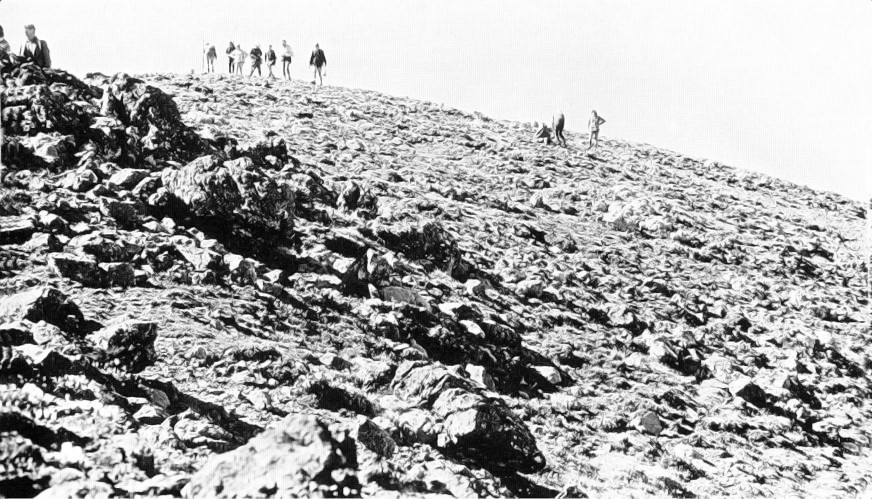
\includegraphics[width=\textwidth]{graphics/fig_105}
	\centering
	\caption[Fellfield on the Black Birch Range]{Fellfield on the Black Birch Range, Marlborough.
	Photo: J. W. Dawson.}%
	\label{fig:105fellfield}
\end{figure}
As a result of the severe environmental conditions in this zone, plants of this type of vegetation are both sparse and specialised.
They are subjected to low average temperatures, heavy frosts, deep snow for part of the year, violent winds, and at times strong sunshine, which may raise the temperature of the extensive areas of exposed rock very considerably.
Erosion by frost action and wind is quite rapid particularly on the greywacke sandstone of the Southern Alps and other axial ranges.
The resulting angular fragments may form a thin layer of debris on ridge crests and sides; but gravity, assisted by wind and, more dramatically, avalanches, constantly moves the products of erosion downslope, so there is little opportunity for the development of even thin soils.
Rock outcrops and bluffs in this zone provide more sheltered and secure sites for plants.
Nevertheless a number of them do establish away from outcrops, especially in deeper debris on moderate to gentle slopes.
Of these, some are small prostrate \BotanicRef{Hebe} shrubs which are also to be found on rock outcrops.
They are not of the whipcord type, but have small rounded leaves arranged in attractive patterns.
\BotanicRef{Hebe haastii}[Hebe][haastii] and \BotanicRef{Hebe epacridea}[Hebe][epacridea]\figureref{\fullref{fig:106hebe}} are yellow or orangey-green; \BotanicRef{Hebe petriei}[Hebe][petriei] is grey-green.
Small herbs are more common --- several diminutive grasses and sedges, and one to several species of \BotanicRef{Epilobium}, \BotanicRef{Ranunculus}, \BotanicRef{Celmisia}, \BotanicRef{Gentiana}, \BotanicRef{Myosotis} and \BotanicRef{Parahebe}.
Small cushion plants also occur; these include \BotanicRef{Hectorella caespitosa}[Hectorella][caespitosa], the softly pubescent species of \BotanicRef{Chionohebe}, \BotanicRef{Phyllachne colensoi}[Phyllachne][colensoi], and sometimes extensive mats of the silver grey \BotanicRef{Celmisia sessiliflora}[Celmisia][sessiliflora] (\IDX{white cushion mountain daisy}).

\begin{SCfigure}[1.5][!b]
	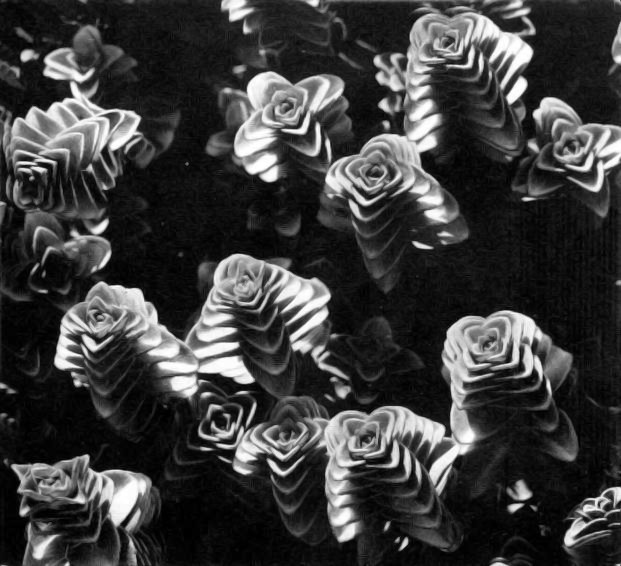
\includegraphics[width=0.5\textwidth]{graphics/fig_106}
	\centering
	\caption[\emph{Hebe epacridea}]{\BotanicRef{Hebe epacridea}[Hebe][epacridea].
	Photo: M. D. King.}%
	\label{fig:106hebe}
\end{SCfigure}

Rooted into clefts of rock outcrops or other stable sites are a number of rather larger and more striking plants.
Hebes are prominent and include both whipcord and non-whipcord species.
Notable among larger herbs are the grey-green, hairy \BotanicRef{Ranunculus buchananii}[Ranunculus][buchananii] with large, white flowers and the yellow-green \IDX{Grahams buttercup} (\BotanicRef{Ranunculus grahamii}[Ranunculus][grahamii]) with large yellow flowers.
The former grows in the south-west of the South island, the latter only in the vicinity of Mt. Cook.\footnote{\cite{wilson1978wild}}
Attractive as well as curious, because of their similarity to the edelweiss of the Swiss Alps, are two species of \BotanicRef{Leucogenes} --- the \IDX{North Island edelweiss} (\BotanicRef{Leucogenes leontopodium}[Leucogenes][leontopodium]) throughout the North Island and the northeastern South Island and the smaller leaved \IDX{South Island edelweiss} \BotanicRef{Leucogenes grandiceps}[Leucogenes][grandiceps] throughout the South Island and Fiordland.
The flowers of both species are white and woolly with yellow to orange centres.

Most outstanding in these situations, however, are a number of large cushion plants, some of which, because of their hummocky form and woolly pubescence, are known as `vegetable sheep'.
These larger cushion plants are extremely firm in texture and sometimes a metre or more in diameter.
The vegetable sheep belong to the daisy family (Compositae) and they are essentially shrubs --- as is evidenced by the tortuous woody stems revealed by the erosion of dead plants.
The living leaves of branch tips at the cushion surface closely invest one another as permanent buds, while the dead interior leaves break down into a blotting paper-like, water retentive mass, which fills the spaces between the branches.
The Canterbury \IDX{vegetable sheep} (\BotanicRef{Raoulia eximia}[Raoulia][eximia]), found on drier eastern mountains from mid-Canterbury to north Otago, is grey-green in colour and the velvety leaf buds are often compressed into more or less hexagonal shapes.
Several other species of \BotanicRef{Raoulia} form smaller cushions in fellfield\figureref{\fullref{fig:107fellfield-rock}}.
\begin{SCfigure}[1.0][!b]
	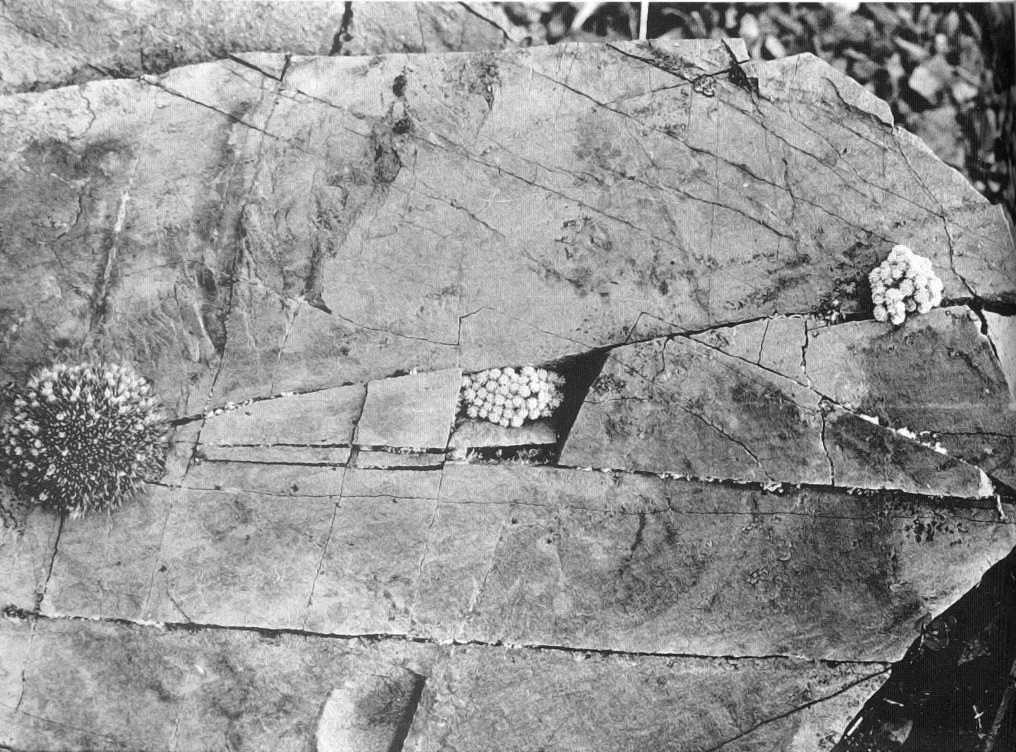
\includegraphics[width=0.66\textwidth]{graphics/fig_107}
	\centering
	\caption[A rock in fellfield on the crest of the St.\ Arnaud Range]{A rock in fellfield on the crest of the St.\ Arnaud Range, northern South Island.
	Frost action has formed fissures in the rock where small cushions of \BotanicRef{Colobanthus canaliculatus}[Colobanthus][canaliculatus] (left) and \BotanicRef{Raoulia bryoides}[Raoulia][bryoides] (centre and right) have established.
	Photo: J. W. Dawson.}%
	\label{fig:107fellfield-rock}
\end{SCfigure}
The more handsome (in my view) Marlborough \IDX{vegetable sheep} (\BotanicRef{Haastia pulvinaris}[Haastia][pulvinaris]) is restricted to the drier mountains of the north east of the South Island.
The large cushions are buff to pale yellow in colour and the leaf buds are larger and woollier than those of the raoulias\figureref{\fullref{fig:108vegetable-sheep}, \fullref{fig:109haastia}}.

\begin{figure}[!t]
	% Outer minipage scaled to limit width.
	% Inner minipages scaled so the images have the same height.
	\begin{minipage}[t]{\textwidth}
		\begin{minipage}[t]{(\textwidth-\fgap) * \real{0.496}}
			\centering
			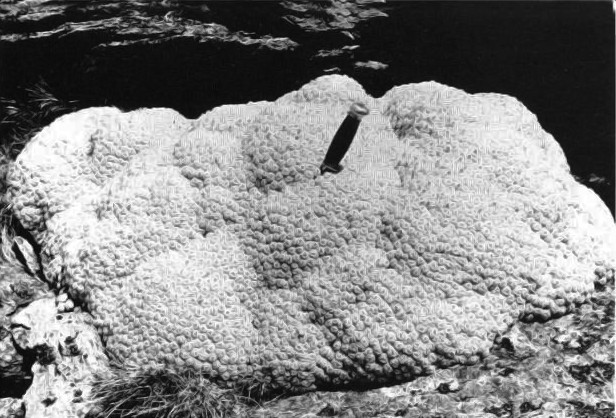
\includegraphics[width=\textwidth]{graphics/fig_108}
			\caption[Large cushion of the Marlborough vegetable sheep]{Large cushion of the Marlborough vegetable sheep, \BotanicRef{Haastia pulvinaris}[Haastia][pulvinaris].
			Mt. Cupola, Nelson Lakes National Park.
			Photo: J. W. Dawson.}%
			\label{fig:108vegetable-sheep}
		\end{minipage}\hspace{\fgap}%
		\begin{minipage}[t]{(\textwidth-\fgap) * \real{0.504}}
			\centering
			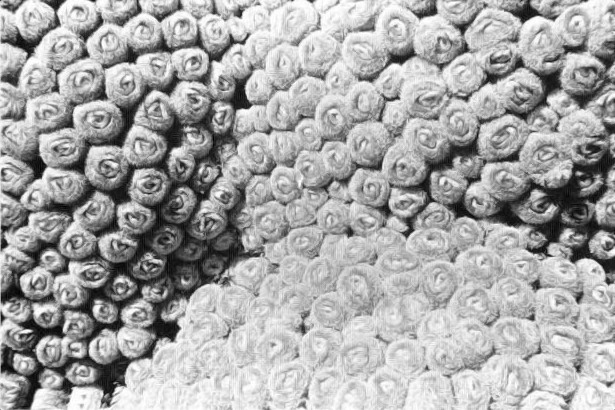
\includegraphics[width=\textwidth]{graphics/fig_109}
			\caption[Close view of a portion of a \emph{Haastia pulvinaris}]{Close view of a portion of a \BotanicRef{Haastia pulvinaris}[Haastia][pulvinaris] cushion showing the branchlet tips closely invested by woolly leaves.
			Photo: J. W. Dawson.}%
			\label{fig:109haastia}
		\end{minipage}
	\end{minipage}
\end{figure}

Two spaniards (\BotanicRef{Aciphylla}) are notable cushion plants in fellfield.
\IDX{Dobsons speargrass} (\BotanicRef{Aciphylla dobsonii}[Aciphylla][dobsonii]) in South Canterbury and North Otago may form perfectly hemispherical cushions more than half a metre in diameter\figureref{\fullref{fig:110cushion-spaniard}}, while \BotanicRef{Aciphylla simplex}[Aciphylla][simplex] of Central Otago forms somewhat smaller cushions.
Both species have thick, rigid leaves coloured bright orange-yellow.
\begin{SCfigure}[2.0][t]
	\centering
	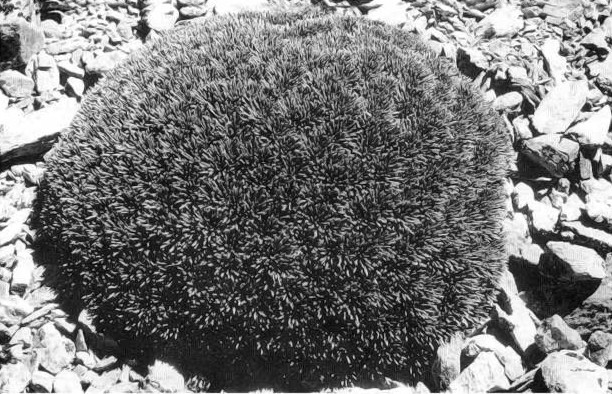
\includegraphics[width=0.66\textwidth]{graphics/fig_110}
	\caption[Hemispherical cushion of the cushion spaniard]{Hemispherical cushion of the cushion spaniard, \BotanicRef{Aciphylla dobsonii}[Aciphylla][dobsonii].
	Mt. St.\ Bathans, Otago.
	Photo: J. W. Dawson.}%
	\label{fig:110cushion-spaniard}
\end{SCfigure}

The two flowering plants of fellfield which hold the altitude record are \BotanicRef{Hebe haastii}[Hebe][haastii] and \IDX{Birleys veronica} \BotanicRef{Parahebe birleyii}[Parahebe][birleyii], both having been recorded at \SI{2900}{\metre} in the Mt. Cook region.\footnote{\cite{wilson1978wild}}
At \SI{2800}{\metre} \IDX{Grahams buttercup} (\BotanicRef{Ranunculus grahamii}[Ranunculus][grahamii]) is not far behind.
Above these altitudes only lichens and mosses cling to steep rocky faces in the zone of permanent snow.

\section{Scree Plants}

Screes or shingle slips might be regarded as a very special type of fellfield.
They are widespread on the drier eastern mountains of Canterbury and Marlborough and some mountain peaks may have their mid and lower slopes completely buried in deep aprons of angular stones through several thousand metres of altitude\figureref{\fullref{fig:111craigieburn}}.
\begin{figure}[t]
	\centering
	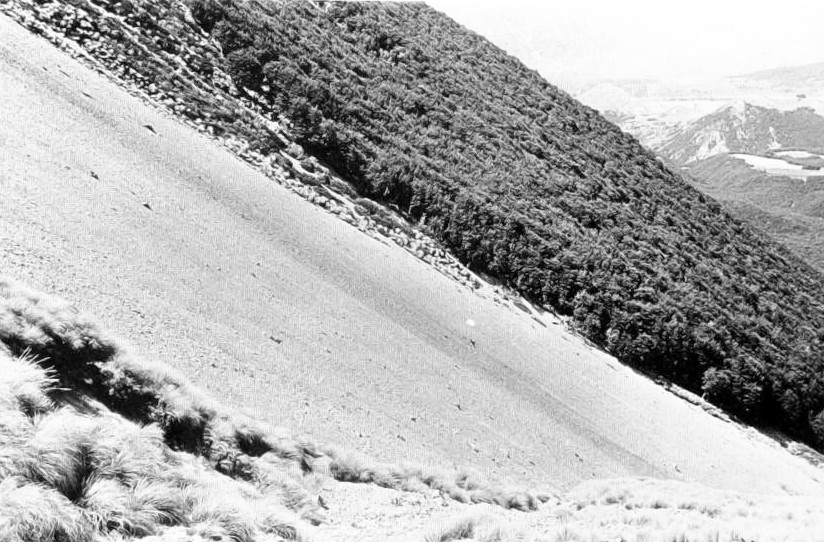
\includegraphics[width=\textwidth]{graphics/fig_111}
	\caption[A steep scree on the Craigieburn Range]{A steep scree on the Craigieburn Range, Canterbury.
	The forest is of \IDX{mountain beech} (\BotanicRef{Nothofagus solandri var.\ cliffortioides}[Nothofagus][solandri var.\ cliffortioides]).
	Photo: J. W. Dawson.}%
	\label{fig:111craigieburn}
\end{figure}
These vast accumulations result from the already mentioned rapid disintegration of greywacke under high alpine conditions, and the relatively slow downward movement of the rock fragments in the absence of heavy rainfall.

The screes are poised at the angle of rest and are very difficult to traverse as the weight of a person will tip the balance and set the stones in motion.
Altogether the screes seem an improbable habitat for plants.
Apart from their instability, the stones appear soil-less and arid and when the sun shines they can become very hot, raising the temperature of the air directly above very considerably.
In fact when one manages to get out onto a scree it seems at first to be entirely plantless, then one small plant is spotted, then another and another.
The plants are often grey like the stones, fleshy, and tend to be scattered fairly evenly across the scree several metres apart.
At first they all appear the same, but closer inspection reveals several different and mostly quite unrelated species.
About a dozen of these are found only on screes and there only away from the margins, in the deeper and most mobile parts.
It is clear then that conditions are not as impossible as they seem.
Beneath the surface the stones diminish in size quite rapidly to a sandy soil at a depth of about \SIrange{40}{50}{\centi\metre}.
The extensive root systems of the plants, arising directly from the bases of leaf rosettes or from spreading rhizomes, branch widely through this soil, which is constantly wet from water seeping downslope.
Thus scree plants do not in fact have a water problem, even when high temperatures at the scree surface lead to excessive water loss from the leaves.
So far, so good, but what about the instability problem? If a plant is lucky the scree will not move in its vicinity during the growing season, but if it does the scree plants are adapted to survive the event.
If the layer of stones above the soil moves substantially, although the leaves and flowers or flower heads of a scree plant will be either buried or sheared off, its root system and rootstock or rhizome will survive intact and will be able to replace the lost parts.
In some scree species the leaf petioles and flower stalks taper downwards so that their connections with the rootstock are almost threadlike and can break fairly readily.
If these connections were thick and tough then the whole plant might be uprooted and die.
The notable example of this type is \BotanicRef{Lignocarpa carnosula}[Lignocarpa][carnosula], a grey-green, fleshy plant with much divided leaves, which belongs to the carrot family (Umbelliferae).
Its dry seed heads break off at the weak connection and blow around on the scree surface like a tumbleweed, scattering seeds as they go.

The best known scree species is the \IDX{penwiper} (\BotanicRef{Notothlaspi rosulatum}[Notothlaspi][rosulatum])\figureref{\fullref{fig:112penwiper}}, which belongs to the cabbage family (Cruciferae).
\begin{SCfigure}[2.0][!b]
	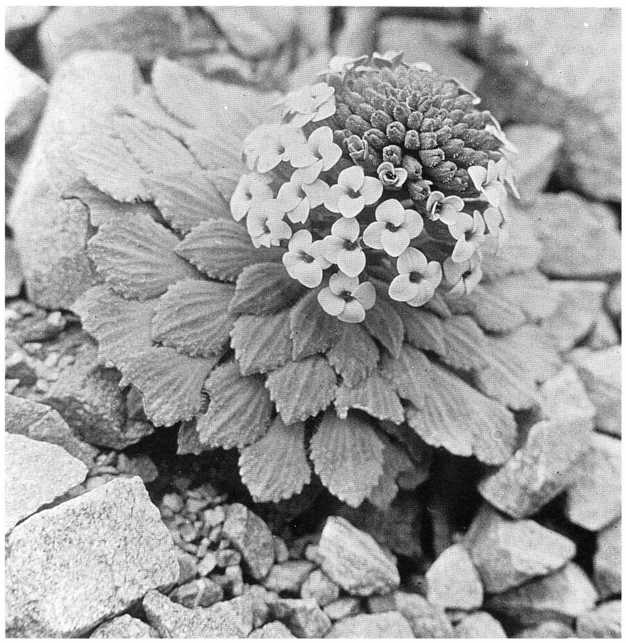
\includegraphics[width=0.5\textwidth]{graphics/fig_112}
	\centering
	\caption[The penwiper plant]{The penwiper, \BotanicRef{Notothlaspi rosulatum}[Notothlaspi][rosulatum].
	Porter's Pass, Canterbury.
	Photo: J. W. Dawson.}%
	\label{fig:112penwiper}
\end{SCfigure}
Its rosettes of grey, fleshy leaves closely overlap in a dome-like arrangement, which reminded early settlers of the similarly arranged and sewn together diamonds of felt on which they wiped their quill pens.
The quite large flowers in massed heads are ivory in colour and have a very strong perfume reminiscent of stock in the same family.

Other notable plants restricted to mobile screes are \IDX{Haasts buttercup} (\BotanicRef{Ranunculus haastii}[Ranunculus][haastii]) with large yellow flowers, \IDX{scree harebell} (\BotanicRef{Wahlenbergia cartilaginea}[Wahlenbergia][cartilaginea]), and \IDX{scree lobelia} (\BotanicRef{Lobelia roughii}[Lobelia][roughii]), which has distinctive elk's-horn-like leaves with red teeth.
\IDX{Scree chickweed}[scree chickweed] (\BotanicRef{Stellaria roughii}[Stellaria][roughii]) in the chickweed genus is also common, as are two species of \BotanicRef{Leptinella} of which the \IDX{black scree button daisy} (\BotanicRef{Leptinella atrata}[Leptinella][atrata]), with its almost black flowers, is the most remarkable.

The scree endemics die down in winter and most are perennials.
The sole exception is the penwiper, which flowers in its second year then dies.

A number of species common on the more stable parts of screes particularly near the margins are also to be found in ordinary fellfield.
Among these are \IDX{willowherb} (\BotanicRef{Epilobium rubromarginatum}[Epilobium][rubromarginatum]), \IDX{scree poa} (\BotanicRef{Poa buchananii}[Poa][buchananii]) (a grass) and patches of \IDX{bidibid} (\BotanicRef{Acaena glabra}[Acaena][glabra]).
\BotanicRef{Acaena glabra}[Acaena][glabra] belongs to the bidi-bid genus, but its seeds do not have the tiresome habit of attaching themselves to clothing or the wool of sheep, as do those of its more common lowland relatives.
The seeds of \BotanicRef{Acaena glabra}[Acaena][glabra] have spines but these lack hook-like recurved hairs at their tips.
Perhaps the most unusual species in this group is \BotanicRef{Craspedia incana}[Craspedia][incana], a ghost-like plant with all its parts densely clothed in long, white, woolly hairs.

\section{Snow Banks}

At higher altitudes in sheltered hollows, such as cirques or smaller depressions, snow will persist well into the growing season.
Plants growing in such sites must be able to reproduce in just a few months, but they have certain advantages over the plants of the surrounding fellfield.
They have more shelter from gales and, with reduced erosion on their concave slopes, a deeper soil which has a steady if cold supply of water from the gradually melting snow.
The flowers of some of the snow bank plants may actually open beneath the melting snow.
This is the case for two species of \BotanicRef{Caltha} with their Ranunculus-like flowers, those of \IDX{white caltha} (\BotanicRef{Caltha obtusa}[Caltha][obtusa]) being white and \IDX{marsh marigold} (\BotanicRef{Caltha novae-zelandiae}[Caltha][novae-zelandiae]) yellow.
Snowbank plants form a continuous sward, with the \IDX{snow patch grass}, \BotanicRef{Chionochloa oreophila}[Chionochloa][oreophila], usually predominating.
Among other prominent plants are \IDX{silky alpine buttercup} (\BotanicRef{Ranunculus sericophyllus}[Ranunculus][sericophyllus]) with deeply divided leaves and relatively large yellow flowers; \BotanicRef{Celmisia allanii}[Celmisia][allanii], with patch forming rosettes of fluffy pale grey to snow white leaves; the related but pale green \BotanicRef{Celmisia haastii}[Celmisia][haastii], and two mat forming species, which although flowering plants look remarkably like mosses --- \IDX{scabweed} (\BotanicRef{Raoulia subulata}[Raoulia][subulata]) and \BotanicRef{Drapetes lyallii}[Drapetes][lyallii].

\section[Cushion Moorland]{Cushion Moorland\thinspace\footnote{\cite{mark1970high}}}

Most New Zealand mountains are steep with narrow ridges and distinct peaks, but in central and north Otago in the south of the South Island there are a number of quite different block mountains, bounded by faults, with flat, plateau-like summits dotted with prominent rocky tors\figureref{\fullref{fig:113summit}}.
\begin{figure}[t]
	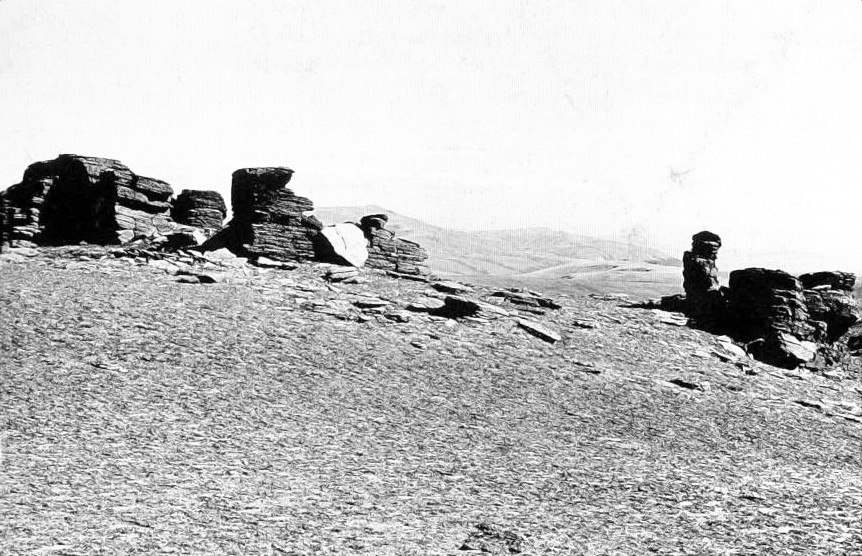
\includegraphics[width=\textwidth]{graphics/fig_113}
	\caption[Summit of the Old Man Range]{Summit of the Old Man Range, Central Otago.
	The surface in the foreground and back to the tors is almost completely covered with cushion moorland.
	Photo: J. W. Dawson.}%
	\label{fig:113summit}
\end{figure}
During the last glaciation when the winds were strong and much of the landscape was open with little plant cover, dust storms would have been frequent and sometimes quite deep deposits of dust, known as loess, would have built up on the hills and mountains.
On the loess mantling the flat tops of the Otago mountains, cushion moorland forms a low but more or less continuous cover.
Conditions here are at least as severe as those of the fellfield, with strong, cold gales from the south, heavy snow in winter and frequent severe frosts.
Over a 5 year period on the Old Man Range at \SI{1590}{\metre} there were on average 113 ice days, 179 freeze-thaw days and only 73 frost-free days per year.

In this type of vegetation small cushion plants are characteristic, with \IDX{cushion inaka} (\BotanicRef{Dracophyllum muscoides}[Dracophyllum][muscoides]) the most common, but also the silvery \BotanicRef{Raoulia hectorii}[Raoulia][hectorii], \BotanicRef{Anisotome imbricata}[Anisotome][imbricata] (Umbelliferae) with dense silver-grey hairs\figureref{\fullref{fig:114cushion-moorland}} and \BotanicRef{Phyllachne rubra}[Phyllachne][rubra].
\begin{SCfigure}[1.0][!t]
	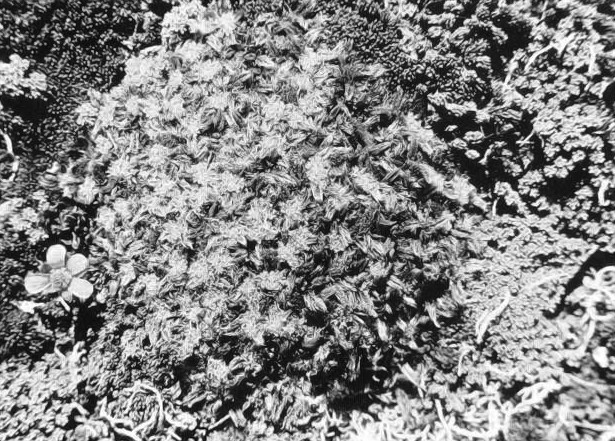
\includegraphics[width=0.66\textwidth]{graphics/fig_114}
	\caption[Close up of cushion moorland]{Close up of cushion moorland.
	A silvery cushion of \BotanicRef{Anisotome imbricata}[Anisotome][imbricata] surrounded by species of \BotanicRef{Dracophyllum} and \BotanicRef{Raoulia}.
	Photo: J. W. Dawson.}%
	\label{fig:114cushion-moorland}
\end{SCfigure}
Small rosette herbs grow in and between the cushions including \BotanicRef{Anisotome lanuginosa}[Anisotome][lanuginosa] (also with dense matted silver-grey hairs obscuring the leaves) and the small spaniard \BotanicRef{Aciphylla hectorii}[Aciphylla][hectorii].
A few small grasses, sedges and luzulas of the rush family may also be present, and small grey lichens are often an important component.

As a result of freeze/thaw action the surface of the cushion moorland is often shaped on level areas into a very regular pattern of hummocks and hollows, which tend to elongate into alternating ridges and trenches on slopes.
